% To je predloga za poročila o domačih nalogah pri predmetih, katerih
% nosilec. Seveda lahko tudi dodaš kakšen nov, zanimiv
% in uporaben element, ki ga v tej predlogi (še) ni. Več o LaTeX-u izveš na
% spletu, na primer na http://tobi.oetiker.ch/lshort/lshort.pdf.
%
% To predlogo lahko spremeniš v PDF dokument s pomočjo programa
% pdflatex, ki je del standardne instalacije LaTeX programov.

\documentclass[a4paper,11pt]{article}
\usepackage{a4wide}
\usepackage{fullpage}
\usepackage[utf8x]{inputenc}
%\usepackage[slovene]{babel}
%\selectlanguage{slovene}
\usepackage[toc,page]{appendix}
\usepackage[pdftex]{graphicx} % za slike
\usepackage{amsfonts}
\usepackage{amsmath}
\usepackage{setspace}
\usepackage{subcaption}
\usepackage{color}
\definecolor{light-gray}{gray}{0.95}
\usepackage{listings} % za vključevanje kode
\usepackage{hyperref}
\renewcommand{\baselinestretch}{1.2} % za boljšo berljivost večji razmak
\renewcommand{\appendixpagename}{Priloge}

\lstset{ % nastavitve za izpis kode, sem lahko tudi kaj dodaš/spremeniš
language=Matlab,
basicstyle=\footnotesize,
basicstyle=\ttfamily\footnotesize\setstretch{1},
backgroundcolor=\color{light-gray},
}

\title{ Topološka analiza podatkov \\ Detekcija oblik}
\author{Špela Čopi and Nika Kastelec }
\date{\today}

\begin{document}

\maketitle

\begin{center}
\textbf{Povzetek}
\end{center}

\begin{center}

V poročilu vam bomo predstavili implementacijo detekcije oblike, ki smo jo izdelali v sklopu predmeta Topološka analiza podatkov. Za vhodne podatke problema smo vzeli množico točk in s pomočjo različnih topoloških prijemov določili ali predstavlja katero izmed vnaprej izbranih oblik. Reševanje problema temelji na določanju homološke grupe vhodnih podatkov s pomočjo obstojne topologije (\textit{perisitance topology}), gradnje Vietris-Rips kompleksa in izračunavo Bettijevih števil.

\end{center}


\section{Uvod}

Problem prepoznavanja oblik je bil v nalogi skrčen na prepoznavanje določenih oblik. To so disk, črta, krožnica, sfera in torus. Te oblike po večini spadajo v različne homološke grupe, zato smo iskali postopek za določanje homoloških grup. Odločili smo se za izgradnjo Vietoris-Rips kompleksov in računanje Betti števil pri različnih razdaljah med točkami. Na podlagi spreminjanja stevila komponent, lukenj in votlin smo nato določili homološko grupo. 
V drugem koraku smo morali ločiti med črto in diskom, ker oba spadata v isto homološko grupo. Tega smo se lotili z iskanjem preseka med sfero in črto oziroma diskom, ki ga nato odstranimo od sfere. 

\section{Podatki}

Vhodne podatke smo izdelali s pomočjo porgrama Blender za 3D modeliranje. V programu smo zmodelirali disk, črto, krožnico, sfero in torus ter iz njih pridobili množice točk. Velikost vhodnih podatkov (oziroma število točk v množici) je bilo zaradi slabše učinkovitostji implementacije nekoliko omejeno navzdol. 

\begin{figure}[h]
\centering
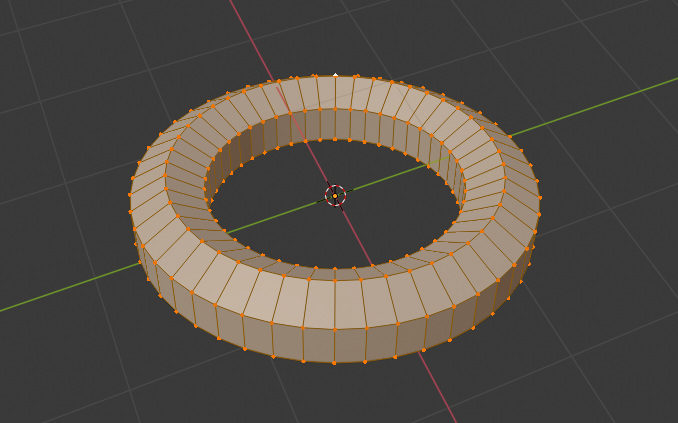
\includegraphics[width=0.4\textwidth]{blender_torus}
\caption{Primer modela v programu Blender.}
\end{figure}
  
Imeli smo učno in testno množico. Razlike med učnimi in testnimi modeli so bile v velikosti, poziciji in rotaciji.

\section{Metode}

\subsection{Izgradnja Vietoris-Rips kompleksa}

Pri izgradnji Vietoris-Rips kompleksa je pomembno kako izberemo interval is katerega vzemamo $\epsilon$-e (razdaljo za grajenje kompleka). V teoriji bi interval izbrali tako, da bi za posamezen objekt avtomatično izbrali interval, kjer se Bettijeva števila spreminjajo. Ker implementiran algoritem ni dovolj učinkovit in je prepočasen za velike $\epsilon$-e, sva interval izbirali empirično. Za naše učne primere $\epsilon$ vzamemo iz intervala $(0, 1)$.





\subsection{Bettijeva števila}
Bettijeva števila $\beta_i$ smo za posamezni Vietoris-Rips kompleks izračunali s pomočjo knjižnice \texttt{mogutda}. Ker so vsi zadani primeri vloženi v tri demenzionalni prostor, smo za vsak kompleks izračunali le $\beta_0$, $\beta_1$ in $\beta_2$. \par
Tako za vsak oblak točk, za katerega želimo prepoznati obliko, dobimo tabelo s tremi stolpci (za vsako Bettijevo  število) in $j$ vrsticami, kjer je $j$ število Vietoris-Rips kompleksov, ki smo jih zgradili.\par
Potem iz danih stolpcev zgoraj opisane tabele razberemo prevladujoče Bettijevo število. To naredimo tako, da najprej preštejemo število zaporednih ponovitev. Nato za vsako izračunamo kakšen procent vseh izračunanih predstavlja. Na koncu izberemo tisto število, ki zadošča pogojou o dovolj velikem odstotku zaporednih ponovitev in in je hkrati največje od takih. Na tak način izbiramo  zato, ker se zelo velika števila pojavijo malokrat, poleg želenih razultatov pa se velikokrat ponovi $0$, ki se pojavi kadar se različno deminzjonalne luknje zapolnijo (v zadnjih vrsticah) in preden se luknje v drugih dimenzijah pokažejo (v začetnih vrsticah, ko ima kompleks še veliko komponent). Ta način ni najbolj učinkovit, ampak deluje na izbranih oblikah. \par



\subsection{Prepoznavanje modelov iz iste homološke grupe}

Ker imata črta in disk obe eno komponento, nič lukenj in nič votlin, se njuna Bettijeva števila ujemajo, dbimo vrednosti $\beta_0=1$, $\beta_1=0$ in $\beta_2=0$. Da lahko črto in disk razločimo, konstruiramo oblak točk, ki predstavlja sfero, nato pa od nje izločimo točke, ki so blizu prvotnega oblaka točk (črta ali disk). Tu moramo biti pozorni, da sfera ni prevelika in da je prav postavljena v prostor. Potem na sferi brez izbranih točk ponovno kličemo algoritem za prepoznavo oblik in v primeru, da algoritem prepozna $2$ komponenti (torej je disk razdelil sfero na dva dela) lahko sklepamo, da je prvotni oblak točk predstavljal disk, če pa je prepoznal eno komponento z dvema $1$-dimenzijonalnima luknjama (torej črta prebode sfero na dveh mestih) lahko sklepamo, da je prvotni oblak točk predstavljal črto. Pri tem moramo biti pozorni na to, da je gostota točk na modelu (črta, disk) dovolj velika, da je razdalja med modelom in sfero pravilno izračunana.

\section{Rešitve}
Metodo stestiramo na učnih in nekaj testnih primerih. Z nekaj ročne pomoči pri določanju intervalov za gradnjo Vietoris-Rips kompleksov je program za vse modele izpisal pravilno rešitev. \par
Oglejmo si nekaj vhodnih in ishodnih podatkov:
    \begin{figure}[h!]
        \centering
        \begin{subfigure}[b]{0.4\linewidth}
          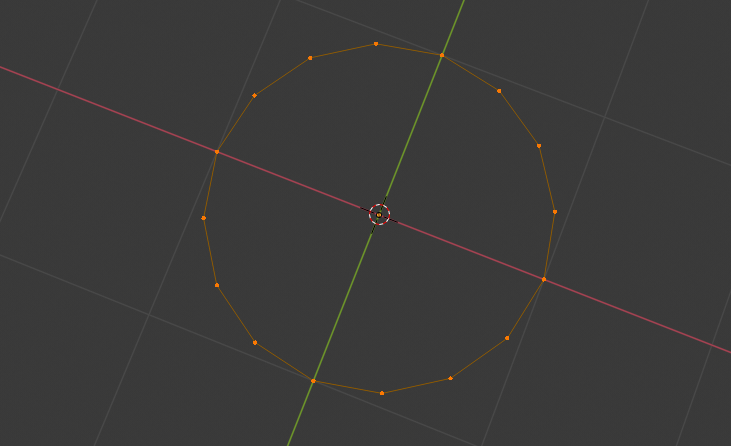
\includegraphics[width=\linewidth]{circle.png}
          \caption{Model krožnice v Blanderju}
        \end{subfigure}
        
        \begin{subfigure}[b]{0.2\linewidth}
          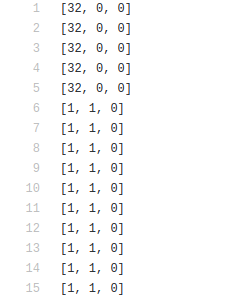
\includegraphics[width=\linewidth]{circle_betti.png}
          \caption{Bettijeva števila pri različnih $\epsilon$-ih, iz katerih algoritem izračuna $1$, $1$, $0$}
        \end{subfigure}
        
      \end{figure}
      
    \begin{figure}[h!]
        \centering
        \begin{subfigure}[b]{0.4\linewidth}
          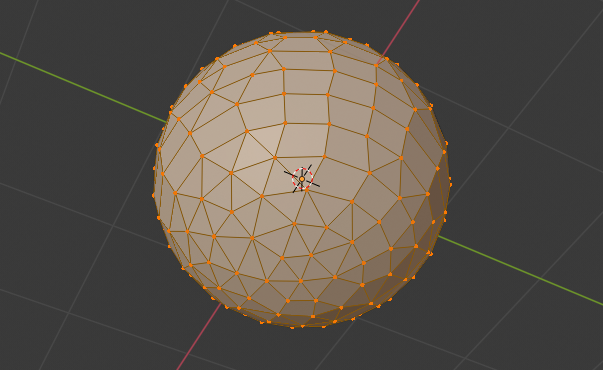
\includegraphics[width=\linewidth]{sphere.png}
          \caption{Model krožnice v Blanderju}
        \end{subfigure}
        \begin{subfigure}[b]{0.2\linewidth}
          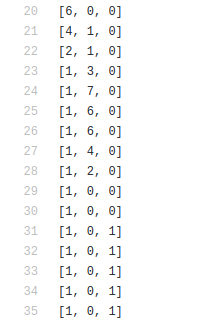
\includegraphics[width=\linewidth]{sphere_betti.png}
          \caption{Bettijeva števila pri različnih $\epsilon$-ih, iz katerih algoritem izračuna $1$, $0$, $1$}
        \end{subfigure}
    
    \end{figure}
    \begin{figure}[h!]
        \centering
        \begin{subfigure}[b]{0.4\linewidth}
          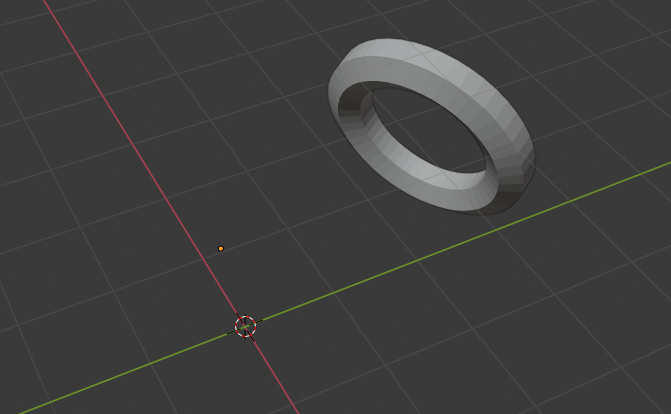
\includegraphics[width=\linewidth]{test_torus.png}
          \caption{Model krožnice v Blanderju}
        \end{subfigure}
        \begin{subfigure}[b]{0.2\linewidth}
          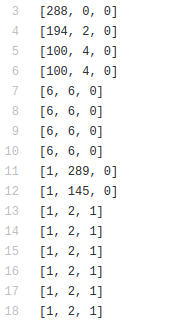
\includegraphics[width=\linewidth]{test_torus_betti.png}
          \caption{Bettijeva števila pri različnih $\epsilon$-ih, iz katerih algoritem izračuna $1$, $2$, $1$}
        \end{subfigure}
        \end{figure}


\newpage
\section{Zaključek}

Program se da izboljšati na več načinov. Lahko bi avtomatizirali izbiro intervala za $\epsilon$ za gradnjo Vietoris-Rips kompleksa tako, da bi brez ročnega nastavljanja dobro prepoznal objekt ne glede na njegove relativne razdalje.\par

Knjižnica mogutda Bettijevih števil morda ni najbol optimalena, saj je časovno zelo potrana, še posebej za $betta_i, i>2$, kar tudi preprečuje prepoznavanje oblik višjih dimenzij. \par

Za boljše določanje Bettijevih števil vhodnih podatkov, bi morali najprej izločiti interval, kjer se število komonent, lukenj in votlin spreminja. Nato pa bi glede na dolžino intervala ter karakteristike sprememb avtomatično določili prag za izbiro Bettijevih števil.

\section{Viri}
https://www.inegi.org.mx/eventos/2014/big-data/doc/P-MichaelLesnick.pdf\\
https://pypi.org/project/mogutda/
\end{document}


